% ------------------------------------------------------------------------------
\section{Triangulations Supporting Efficient Path Traversal}
\label{sec:tins}
% ------------------------------------------------------------------------------

In this section, we describe how our data structures may be used to 
represent triangulations in a manner that permits efficient path
traversal in the EM setting.
In Section \ref{ssec:triangulation_rep}, we describe this representation in the 
general, non-EM setting, giving a compact representation for triangulations 
based on succinct representations of planar graphs.
Later, in Section \ref{ssec:compact_tin_external}, we detail how our succinct
and I/O-efficient planar graph representation can be applied to this representation
to yield a compact representation for 
triangulations permitting I/O-efficient path traversal.

% -------------------------------------------------------------------------
\subsection{Representing Triangulations}
\label{ssec:triangulation_rep}
% -------------------------------------------------------------------------

Let $\pointset$ be a set of points in $\plane$, then the triangulation $\triang$
of $\pointset$ is the planar graph with $\pointset$ vertices and all faces 
(except the outer face) of size $3$.
The set of all edges adjacent to the outer face of the triangulation is the
convex hull of $\pointset$. 
Let $\triang = (\pointset,E,T)$ be the triangulation with vertices $\pointset$, 
edges $E$, and 
triangles (faces) $T$. 
The dual graph of $\triang$ is $\dual{\triang} = (T^*,E^*,\pointset^*)$, it has a node
 $t^* \in T^*$ for each triangle $t \in T$, a face $p^* \in \pointset^*$ for each 
vertex $p \in \pointset$, and an edge $e^* \in E^*$ connecting vertices $t^*_1$ and
 $t^*_2$, if and only if triangles $t_1$ and $t_2$ share an edge in $\triang$.

We further define the \emph{augmented dual graph} 
 $\augdual{\triang} = (\augdual{V} = (\pointset \cup \dual{T}), \augdual{E},
\augdual{F})$.
Figure \ref{fig:aug_tri} shows an example of a triangulation, its dual, 
and its augmented dual graph.
The vertex set of $\augdual{\triang}$ is formed by the union of the vertex set 
$P$ of $\triang$ and the nodes $\dual{T}$ of $\dual{\triang}$. 
We will distinguish between two types of vertices in $\augdual{\triang}$, 
dependening on from which set the vertex is drawn. 
The vertices taken from the dual graph, denoted $\augdual{T}$, 
are referred to as the \emph{triangle nodes}. 
The vertices drawn from the set of vertices in the primal, $\pointset$, 
are refereed   
to as the \emph{point vertices} and are denoted $\augdual{\pointset}$.

For the edges of $\augdual{\triang}$, we again distinguish two types
 of edges. 
The \emph{triangle edges} are exactly the edge set in the dual, $E^*$. 
A \emph{point edge} is added between a triangle node and a point vertex
 if the point vertex is one of the corresponding triangle's three vertices in 
 the primal. 
We denote this set $\augdual{E}$, and define it formally as
$\augdual{E} = \{\augdual{e} | \left( e^* \in E^* \right)
 \cup \left( \augdual{e}=( \augdual{p} \in \augdual{\pointset}, 
  \augdual{t} \in \augdual{T} ) \text{ and } p 
  \text{ adjacent to } t \text{ in } \triang \right) \} $,
where $p$ and $t$ are the vertex and triangle, respectively, corresponding to 
$\augdual{p} \in \augdual{\pointset}$ and $t^{\augdualsym} \in T^{\augdualsym}$. 
$\augdual{\triang}$ also contains a set of faces $F^{\augdualsym}$, but these faces 
do not figure in our discussion. 


For purposes of quantifying bit costs, we denote by $\bitsPerPoint = \OhOf{\lg{N}}$ 
the number of bits required to represent a point in our data structures. 
Many application for triangulations will not require that a key be stored 
with the triangles, so we assume there is no $q$ bit key associated 
with each triangle node. 
We show that the space used by keys in our graph structure is effectively 
the same as the space used by the point set in our triangulation, but that 
if we wish to maintain keys we can do so without significantly increasing 
the space used.

% -------------------------------------------------------------------------------- %
\begin{figure}
\centering
	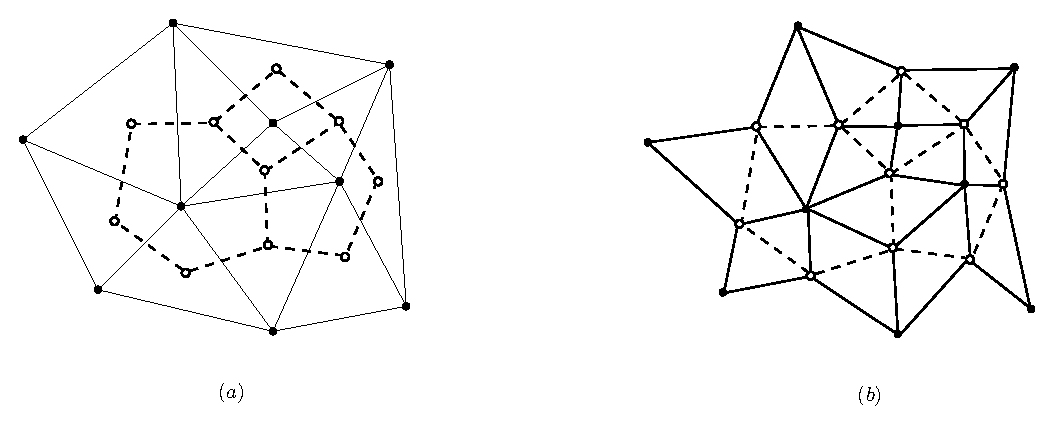
\includegraphics[width=0.8\textwidth]{Fig4}
\caption[Representation of a triangulation as a planar graph]{Representation 
	of a triangulation as a planar graph. 
  (a) The dual graph $\dual{\triang}$ of a triangulation, with vertices as hallow 
circles and edges as dashed lines. 
Edges in the triangulation $\triang$ are shown as solid lines. 
(b) The augmented graph $\augdual{\triang}$ is shown;
hallow points are triangle vertices, solid points are point 
vertices, black dashed lines are triangle edges, and solid lines are point 
edges }\label{fig:aug_tri}
\end{figure}
% ---------------------------------------------------------------------------------%

We begin with the following lemma which we state without proof. 

\begin{lemma}\label{lem:points_for_dual}
Given the dual graph, $\dual{\triang}$ of triangulation $\triang$ with 
$N$ triangles, the augmented dual graph $\augdual{\triang}$ has at most $2N+2$ 
vertices.
\end{lemma}

% Retain this for the THESIS.
%
\begin{proof}
The vertex set $\augdual{V}$ includes the nodes $\dual{T}$, for which 
$|\dual{T}| = N$, and the vertex set $\pointset$. 
We prove by induction that $|P| \le N+2$ and thus $|\augdual{V}| \le 2N + 2$. 
For the base case we have a terrain $\triang$ with a single triangle in which case 
$N = 1$ and $|P| = 3  = N + 2$. 
Now assume that $|P| \le N + 2$ holds for all terrains of $N$ triangles. 
Let $\dual{\triang}_N$ be the dual graph of a triangulation $\triang$ with $N$ 
triangles and $|P|$ vertices. 
The dual graph $\dual{\triang}_{N+1}$ is created by adding a single triangle 
to $\triang$. This new triangle, $t_1$, has three adjacent points, however, 
since $\dual{\triang}_{N+1}$ is connected, at least one dual edge is added 
connecting a vertex $t^*_2 \in \dual{\triang}_N$ with the new vertex 
$t^*_1 \in \dual{\triang}_{N+1}$. 
In $\triang$ this dual edge represents the fact that $t_1$ and $t_2$ are 
adjacent, and two of the vertices from $P$ adjacent to $t_2$ are already 
in $\augdual{V}$. Therefore, adding a new triangle adds at most one 
additional point to $\augdual{V}$ and $|\augdual{V}_{N+1}| \le (N+1) + 2$.
\end{proof}

We encode $\augdual{\triang}$ using a succinct planar graph data structure.
The various encodings all involve a permutation of the vertices of 
$\augdual{\triang}$.
Let $\ell(v)$, the \emph{augmented graph label} of $v \in \augdual{V}$, be 
the position of a vertex $v$ in this permutation. 
For every point vertex $p \in \augdual{P} \subset \augdual{V}$ in this set 
we store the point coordinates in an array $\mathcal{P}$ ordered by the 
augmented graph label, $\ell(p)$. 
We create a bit vector $\pi$ of length $|\augdual{V}|$, where 
$\pi[v] = 0$ if $v$ is a triangle vertex and $\pi[v] = 1$ if $v$ is a 
point vertex. 
To summarize this structure we have the following Lemma.

\begin{lemma}\label{lem:terrain_space}
The data structures described above can represent a triangulation, $\triang$, composed 
of $N$ triangles with $\bitsPerPoint = O(\lg{N})$ bit point coordinates, using 
$N\bitsPerPoint + O(N)$ bits, such that given the label of a triangle, the adjacent
 triangles and points can be reported in $O(1)$ time.
\end{lemma}

\begin{proof}
Since the augmented planar graph is simple, we can encode it with 
$2|\augdual{E}| + 2|\augdual{V}| + o(|\augdual{V}|)$ bits 
using the encoding of~\cite{DBLP:journals/siamcomp/ChiangLL05}. 
By Lemma \ref{lem:points_for_dual} if $|\dual{T}| = N$ then 
$|\augdual{V}| \le 2N+2$ which bounds the number of vertices. 
Each triangle node is connected by an edge to at most $3$ 
other triangles, so there are at most $\frac{3}{2} N$ triangle edges. 
Additionally, there are $3N$ point edges connecting the 
triangle vertices with point vertices, so in total there are no 
more than $\frac{9}{2}N$ edges. 
Thus the augmented graph can be encoded using at most $13N + o(N)$ bits. 

In~\cite{DBLP:journals/siamcomp/ChiangLL05} adjacency and degree queries
 can be performed in $O(1)$ time. 
We must still demonstrate that given a label we can identify the corresponding 
triangle vertex, and show that for a vertex we can distinguish between point 
vertex and triangle node neighbours. 
We assign to each triangle a unique graph label as follows. 
Consider the set of triangles in $\triang$, the graph label of each 
triangle corresponds to that of its dual vertex $t^* \in T^*$. 
In $\augdual{\triang}$ each of these vertices has an augmented graph label.  
The graph label of dual node $\dual{t} \in \dual{T}$, and therefore the 
corresponding triangle, is equal to the rank of the corresponding 
triangle vertex, $\augdual{t}$'s augmented graph label among all 
vertices from the set $\augdual{t}$. 

Given the graph label of a triangle node $\augdual{t} \in \augdual{T}$,
 the augmented graph label is calculated as $\ell(t^{\augdualsym}) = 
\selop[0]{\pi, \augdual{t}}$.
Conversely, given $\ell(\augdual{t})$ for a triangle vertex 
$\augdual{t} \in \augdual{T}$, we can report the graph label 
of $\augdual{t}$ by $\rankop[0]{\pi,\ell(\augdual{t})}$. 
To report the triangles adjacent to $\augdual{t}$, we check in 
the succinct encoding for $\augdual{\triang}$ to find all neighbours of 
$\augdual{t}$. 
Since $d \le 6$, this operation takes constant time. 
Let $\augdual{v} \in \augdual{V}$ be a neighbour of $\augdual{t}$ in 
$\augdual{\triang}$. 
The value of $\pi[\augdual{v}]$ indicates whether $\augdual{v}$ is a 
triangle node or point vertex. 
We can recover the coordinates of a point vertex $\augdual{v}$ by 
$\mathcal{P}[\rankop[1]{\pi,\augdual{v}}]$.

The array $\mathcal{P}$ stores at most $N+2$ points. 
If each point requires $\bitsPerPoint$ bits then $\mathcal{P}$ 
requires $N\bitsPerPoint$ bits. 
Finally, by Lemma \ref{lem:rank_select}(b) we can store the bit array 
$\pi$ such that $\rankop$ and $\selop$ can be performed in constant time 
with $N + o(N)$ bits.
\end{proof}

% -------------------------------------------------------------------------
\subsection{Compact External Memory Representation}
\label{ssec:compact_tin_external}
% -------------------------------------------------------------------------

In this section we extend our data structures for I/O efficient traversal in 
bounded degree planar graphs (Section \ref{sec:graph_rep}) to triangulations. 
We thereby obtain a triangulation that is compact, but which also 
permits efficient traversal. 
We represent $\triang$ by its dual graph $\dual{\triang}$. 
Since the dual graph of the the triangulation (and subsequently each component) is a 
bounded degree planar graph, it can be represented with the data structures 
described in Section \ref{sec:graph_rep}. 
Each component is a subgraph of $\dual{\triang}$, for which we generate the 
augmented subgraph, as described in Section~\ref{ssec:triangulation_rep}.

\begin{lemma}\label{lem:terrain_components}
The space requirement, in bits, to store a component ($\alpha$-neighbour-hood
 or sub-region) representing a triangulation is within a constant factor of the 
space required to store the triangulation's dual graph. 
\end{lemma}

\begin{proof}
We first consider the case of $\alpha$-neighbourhoods. 
To store a triangulation we require additional space to store: the points in $P$ 
adjacent to the component's triangles, the augmented 
graph, which includes more vertices and edges, and the bit-vector $\pi$. 
By Lemma~\ref{lem:points_for_dual} the points array is of size at most 
$(\alpha + 2)\bitsPerPoint$ bits. 
Since the $\alpha \bitsPerKey$-bit array of keys is no longer needed, storing the 
points incurs no additional space over that used to store the dual graph 
in our construction in Section \ref{sec:graph_rep}. 
However, if the keys are needed, we require 
$\alpha (\bitsPerPoint + \bitsPerKey)$ bits to 
store both the points and the key values.  
For the graph representation, again by Lemma \ref{lem:points_for_dual}, in 
the augmented graph we at most double the size of the vertex set and add 
no more than $3 \alpha$ edges. 
The graph encoding is a linear function of the number of edges and 
vertices. 
Therefore, the number of bits required for the graph encoding 
increases by a constant factor. 
Finally for $\pi$ we require fewer than two bits per vertex, so we can add 
this cost to the constant cost of representing the graph.

For sub-regions the analysis is more complex. 
A sub-region may be composed of multiple connected components, thus we cannot 
assume that there will be at most $\succblksize+2$ point vertices in the 
augmented subgraph.  
By Lemma \ref{lem:fred_graph_sep} there are no more than 
$\Theta(N/ \sqrt{\succblksize})$ boundary vertices in $\dual{\triang}$. 
Since each connected component in a sub-region must have at least one boundary vertex, 
this bounds the number of distinct connected components in all sub-regions. 
Each sub-region is composed of at most $\Theta(\sqrt{\succblksize})$ individual 
components, so in the worst case there are no more than 
$\sqrt{\succblksize}( \sqrt{\succblksize} + 2) < 2 \succblksize$ point vertices. 
Thus, the total number of vertices in the augmented graph is less than 
$3\succblksize$ which adds at most an additional $6\succblksize$ edges. 
As demonstrated with the $\alpha$-neighbourhoods, the additional storage, 
for all data structures used to represent a sub-region, 
increases by only a constant factor.
\end{proof}

One important feature of our representation is that each triangle stores 
very limited topological information. 
Consider the information available to some triangle 
$\augdual{t} \in \augdual{T}$ in the augmented dual graph. 
We can determine the - up to three - triangles adjacent to $\augdual{t}$, which 
correspond to the adjacent triangle vertices, as well as the three 
adjacent point vertices, but we have no information about how these are related.  
The only way to acquire this information is to actually visit each of 
$\augdual{t}$'s neighbours and thereby construct the topological 
information. 
Fortunately the need to visit the neighbours of a triangle in order to reconstruct 
its topological information will not increase the I/O costs of path traversal. 
If $\augdual{t}$ corresponds to an interior vertex (in a sub-region), or an 
internal vertex (in an $\alpha$-neighbourhood), then all of its neighbours are 
represented in the current component. 
If $\augdual{t}$ corresponds to a boundary (sub-region) or terminal 
($\alpha$-neighbourhood) vertex then the traversal algorithm already requires 
that a new sub-region, or $\alpha$-neighbourhood, be loaded. 
If we must load an $\alpha$-neighbourhood, then we are ensured all of 
$\augdual{t}$'s neighbours are in the new component. 
In the worst case $\augdual{t}$ is a terminal vertex in a 
$\alpha$-neighbourhood, and a boundary vertex in the newly loaded region. 
This forces us to load a second $\alpha$-neighbourhood, but observe that 
the same sequence of I/Os is necessary even if we were not required to 
reconstruct $\augdual{t}$'s local topology. 
Thus, at no point during a traversal is it necessary to load a component 
merely to construct the topology of a triangle in an adjacent, or overlapping,
component.

Due to Theorem~\ref{thm:planar_graph} and Lemma~\ref{lem:terrain_components} we
have the following theorem.

\begin{theorem}\label{thm:terrain_traversal}
Given triangulation $\triang$, where each point coordinate may be stored in 
$\bitsPerPoint$ bits, there is a data structure that represents $\triang$ in 
$N\bitsPerPoint + O(N) +o(N\bitsPerPoint)$ bits, that permits traversal of a path 
which crosses $K$ faces in $\triang$ with 
$O \left( \frac{K}{ \lg{B} } \right)$ I/O operations.
\end{theorem} 

For the case in which we wish to associate a $q$ bit key with each 
triangle we also have the following theorem.

\begin{theorem}\label{thm:terrain_keys_traversal}
Given triangulation $\triang$, where each point coordinate may be stored 
in $\bitsPerPoint$ bits, and where each triangle has associated with it a 
$\bitsPerKey$ bit key, there is a data structure that represents 
$\triang$ in 
$N(\bitsPerPoint + \bitsPerKey) + O(N) + o(N(\bitsPerPoint + \bitsPerKey))$ bits, that 
permits traversal of a path which crosses $K$ faces in $\triang$ 
with $O \left( \frac{K}{ \lg{B} } \right)$ I/O operations.
\end{theorem}

\begin{proof}
In our proof of Lemma \ref{lem:terrain_components} we demonstrated 
that the number of triangles (dual nodes with an associated $\bitsPerKey$ 
bit key) and points (of $\bitsPerPoint$ bits) are within a constant factor 
of each other in the worst case. 
Assuming this worst case does occur, we are effectively assuming each 
triangle is associated with a $\bitsPerKey$ bit key in our data structures. 
This yields the desired space bound.
\end{proof}

%%% Local Variables:
%%% TeX-PDF-mode: t
%%% TeX-master: "main"
%%% End:
